\documentclass[12pt,reqno]{amsart}
\usepackage[margin=1in]{geometry}
\usepackage{booktabs,url,cleveref}
\usepackage{amsmath}
\usepackage{amssymb}
\usepackage{graphicx}
\usepackage{caption}
\newtheorem{thm}{Theorem}[section]
\newtheorem{prop}[thm]{Proposition}
\newtheorem{lem}[thm]{Lemma}
\newtheorem{cor}[thm]{Corollary}
\usepackage{qtree}
\theoremstyle{definition}
\newtheorem{defn}[thm]{Definition}
\newtheorem{ex}[thm]{Example}

\begin{document}
\title[Catalan Group Midterm Project: Individual Draft]{UCSD Math 184 Spring 2020: \\ Catalan Group Midterm Project \\ Individual Draft}

\author{ARYAMAN P SINGH \\ GROUP R} % Write your name and group letter here

\begin{abstract}
  % Give a brief summary of your document here.
  % Write as if you are speaking to someone outside of Math 184.
  The Catalan numbers are a sequence of natural numbers which appear frequently in various counting problems, as defined in \cite{wiki:catalan}. Professor Richard Stanley described 66 different sets which were counted by the Catalan numbers. 
  
  This paper contains a few examples of, and a combinatorial proof one of these interpretations. It also contains a proof of the generating function for Catalan numbers, and a proof that the Narayana numbers, another sequence of natural numbers like the Catalan number, are positive integers.
\end{abstract}

\maketitle

\section{An interpretation of the Catalan numbers}

\begin{defn}\label{defn:cat.1}
  Exercise 6.19(a) of \cite{MR1676282} (or \cite{stanley_2013}) defines the
  $n$th Catalan number $C_n$ as the number of Subsets $S$ of $\mathbb{N}$ such that $0 \in S$ and such that if $i \in S$ then $i + n, i + n + 1 \in S$
\end{defn}

In other words, the $n$th Catalan number counts the number of subsets $T$ of $\mathbb{N}$ such that $S = \mathbb{N} - T$ still satisfies the conditions $ 0 \in S $ and $ i+n \in S $, $ i+n+1 \in S $ for all $ i \in S $.

Evidently, any such subset $T$ cannot contain any $j$ such that $j \in \{0,n,n+1,2n,2n+1,2n+2,3n,3n+1,3n+2,3n+3,...,\}$. Similarly, for any $i \in S$, $T$ cannot contain any $k$ such that $k \in \{i,i+n,i+n+1,i+2n,i+2n+1,i+2n+2,i+3n,i+3n+2,i+3n+3,...\}$

\subsection{Examples}

For $n=0$ and $n=1$, we can only count the set $\mathbb{N}$.
For $n=2$, we count the sets \(\mathbb{N}, \mathbb{N}-\{1\}\)
For $n=3$, we count the sets \(\mathbb{N}, \mathbb{N} -\{1\}, \mathbb{N} -\{2\}, \mathbb{N} -\{1,2\}, \mathbb{N} -\{1,2,5\}\).

Examples of sets counted are $\mathbb{N} - \{1,2,3,6\}$ for $n=4$, $\mathbb{N} - \{2,3,4,8,9\}$ for $n=5$, $\mathbb{N} - \{1,2,3,4,5,11\}$ for $n=6$


%... Give examples for all n <= 3, and at least 3 examples with n >= 4.
\begin{figure}[h]
  \centering
  \caption{}
  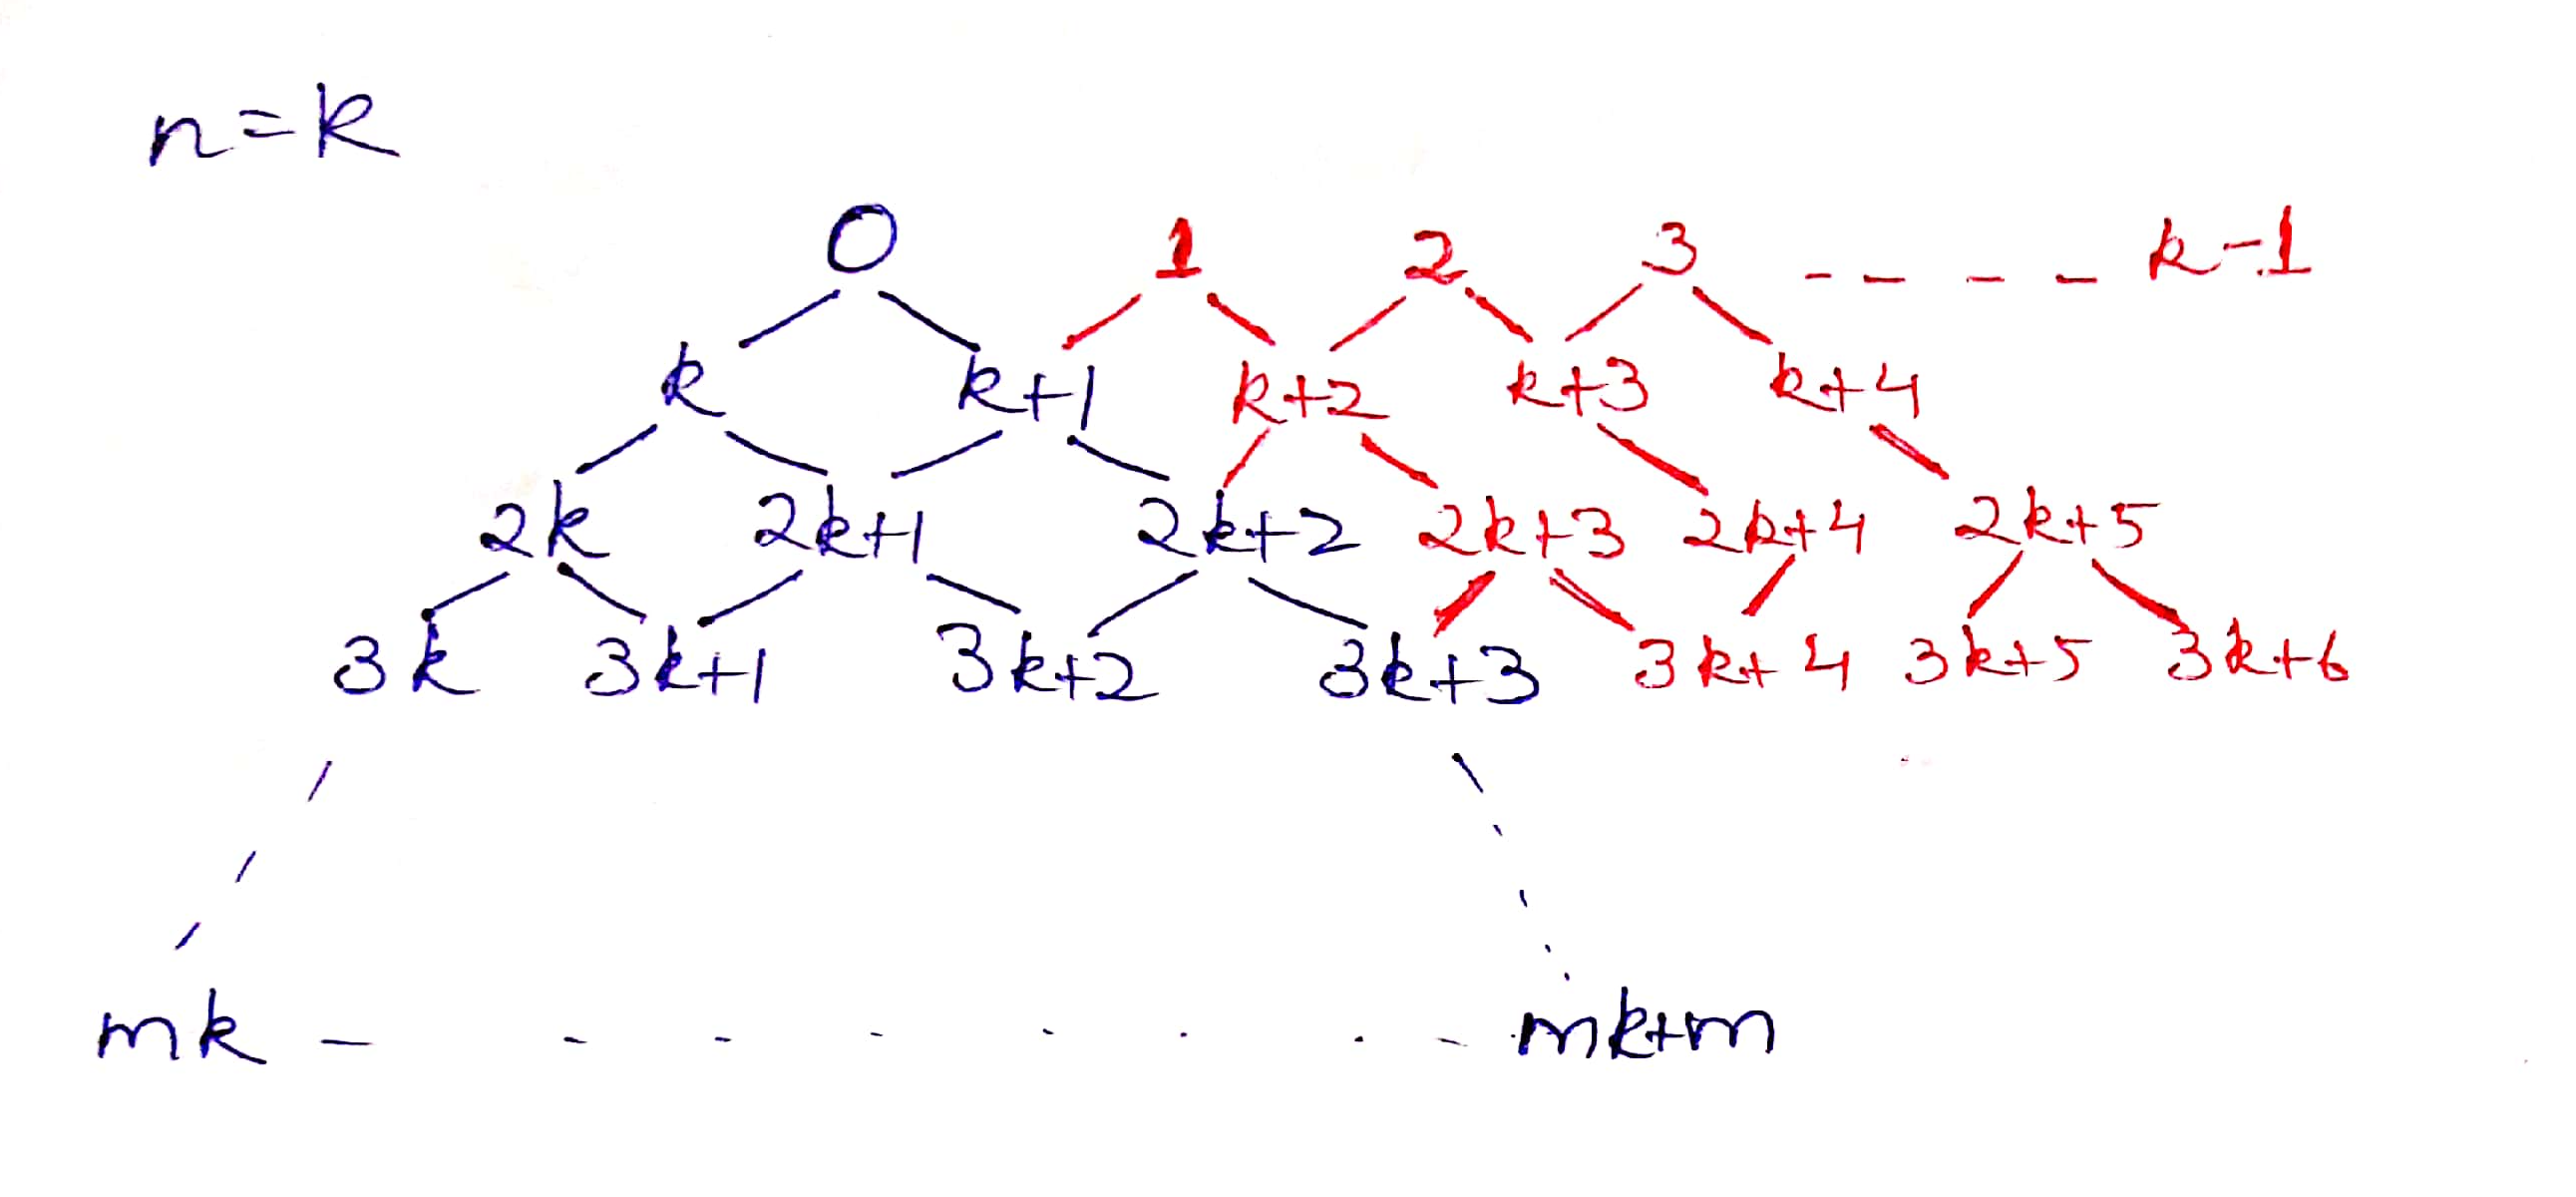
\includegraphics[scale=0.15]{diag-a.png}
  \label{fig:fig1}
  \end{figure}
  
\subsection{Fundamental Catalan Recurrence}

\begin{thm}
  Let $C_n$ be as in \Cref{defn:cat.1}. Then
    \[ C_{n+1} = \sum_{i=0}^n C_i C_{n-i}, \qquad (n \geq 0; C_0 = 1). \]
\end{thm}

\begin{proof}
  %... Give a combinatorial proof that your intepretation satisfies the formula.
  
  
  Consider Figure \ref{fig:fig1} which represents the elements of $\mathbb{N}$ in the form of a tree such that every child node must be in set S if the parent node is in S. Thus, all nodes in blue must be in every subset S for $n=k$, since $0 \in S$ by \textit{\Cref{defn:cat.1}}.
  
  Let T be subsets of $\mathbb{N}$ which are the complement of subsets S being counted in \textit{\Cref{defn:cat.1}}. The number of such sets T is clearly equal to the number of sets S, as by definition $S = \mathbb{N} - T$.
  \begin{figure}[h]
  \centering
  \caption{T(k)}
  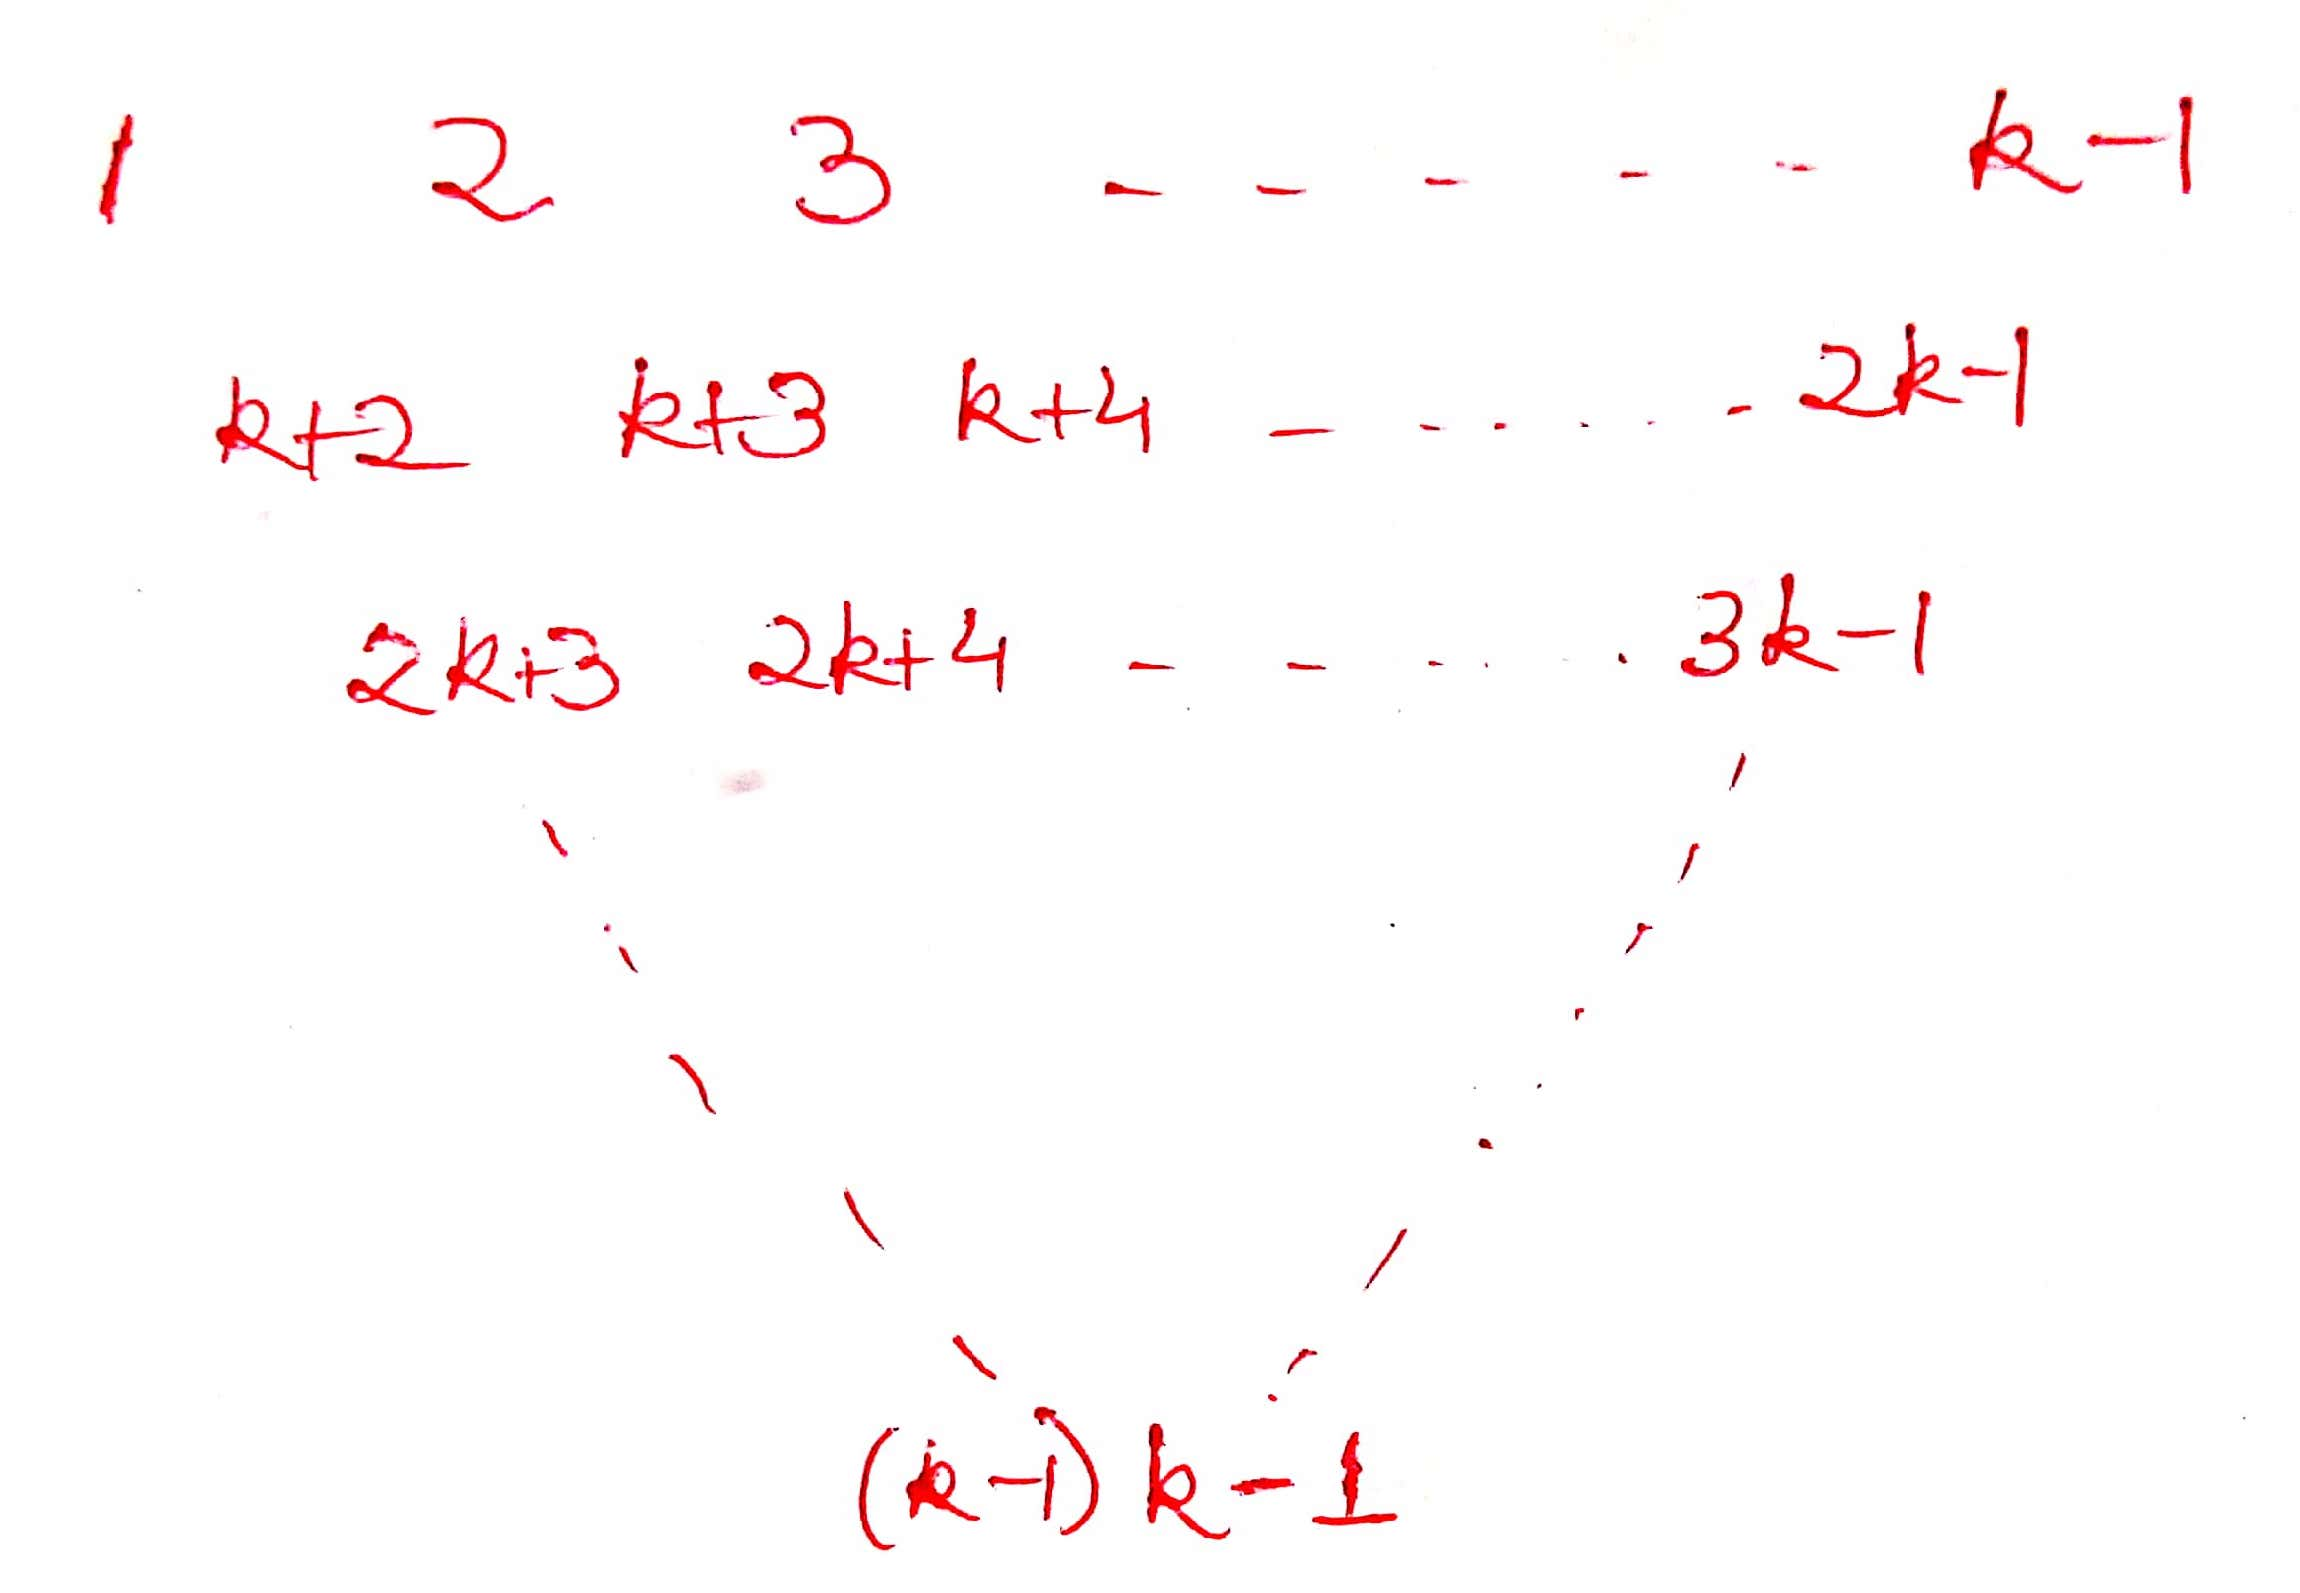
\includegraphics[scale=0.12]{tk.jpg}
  \label{fig:fig2}
  \end{figure}
  \begin{figure}[h]
  \centering
  \caption{Picking subsets of T(n+1)}
  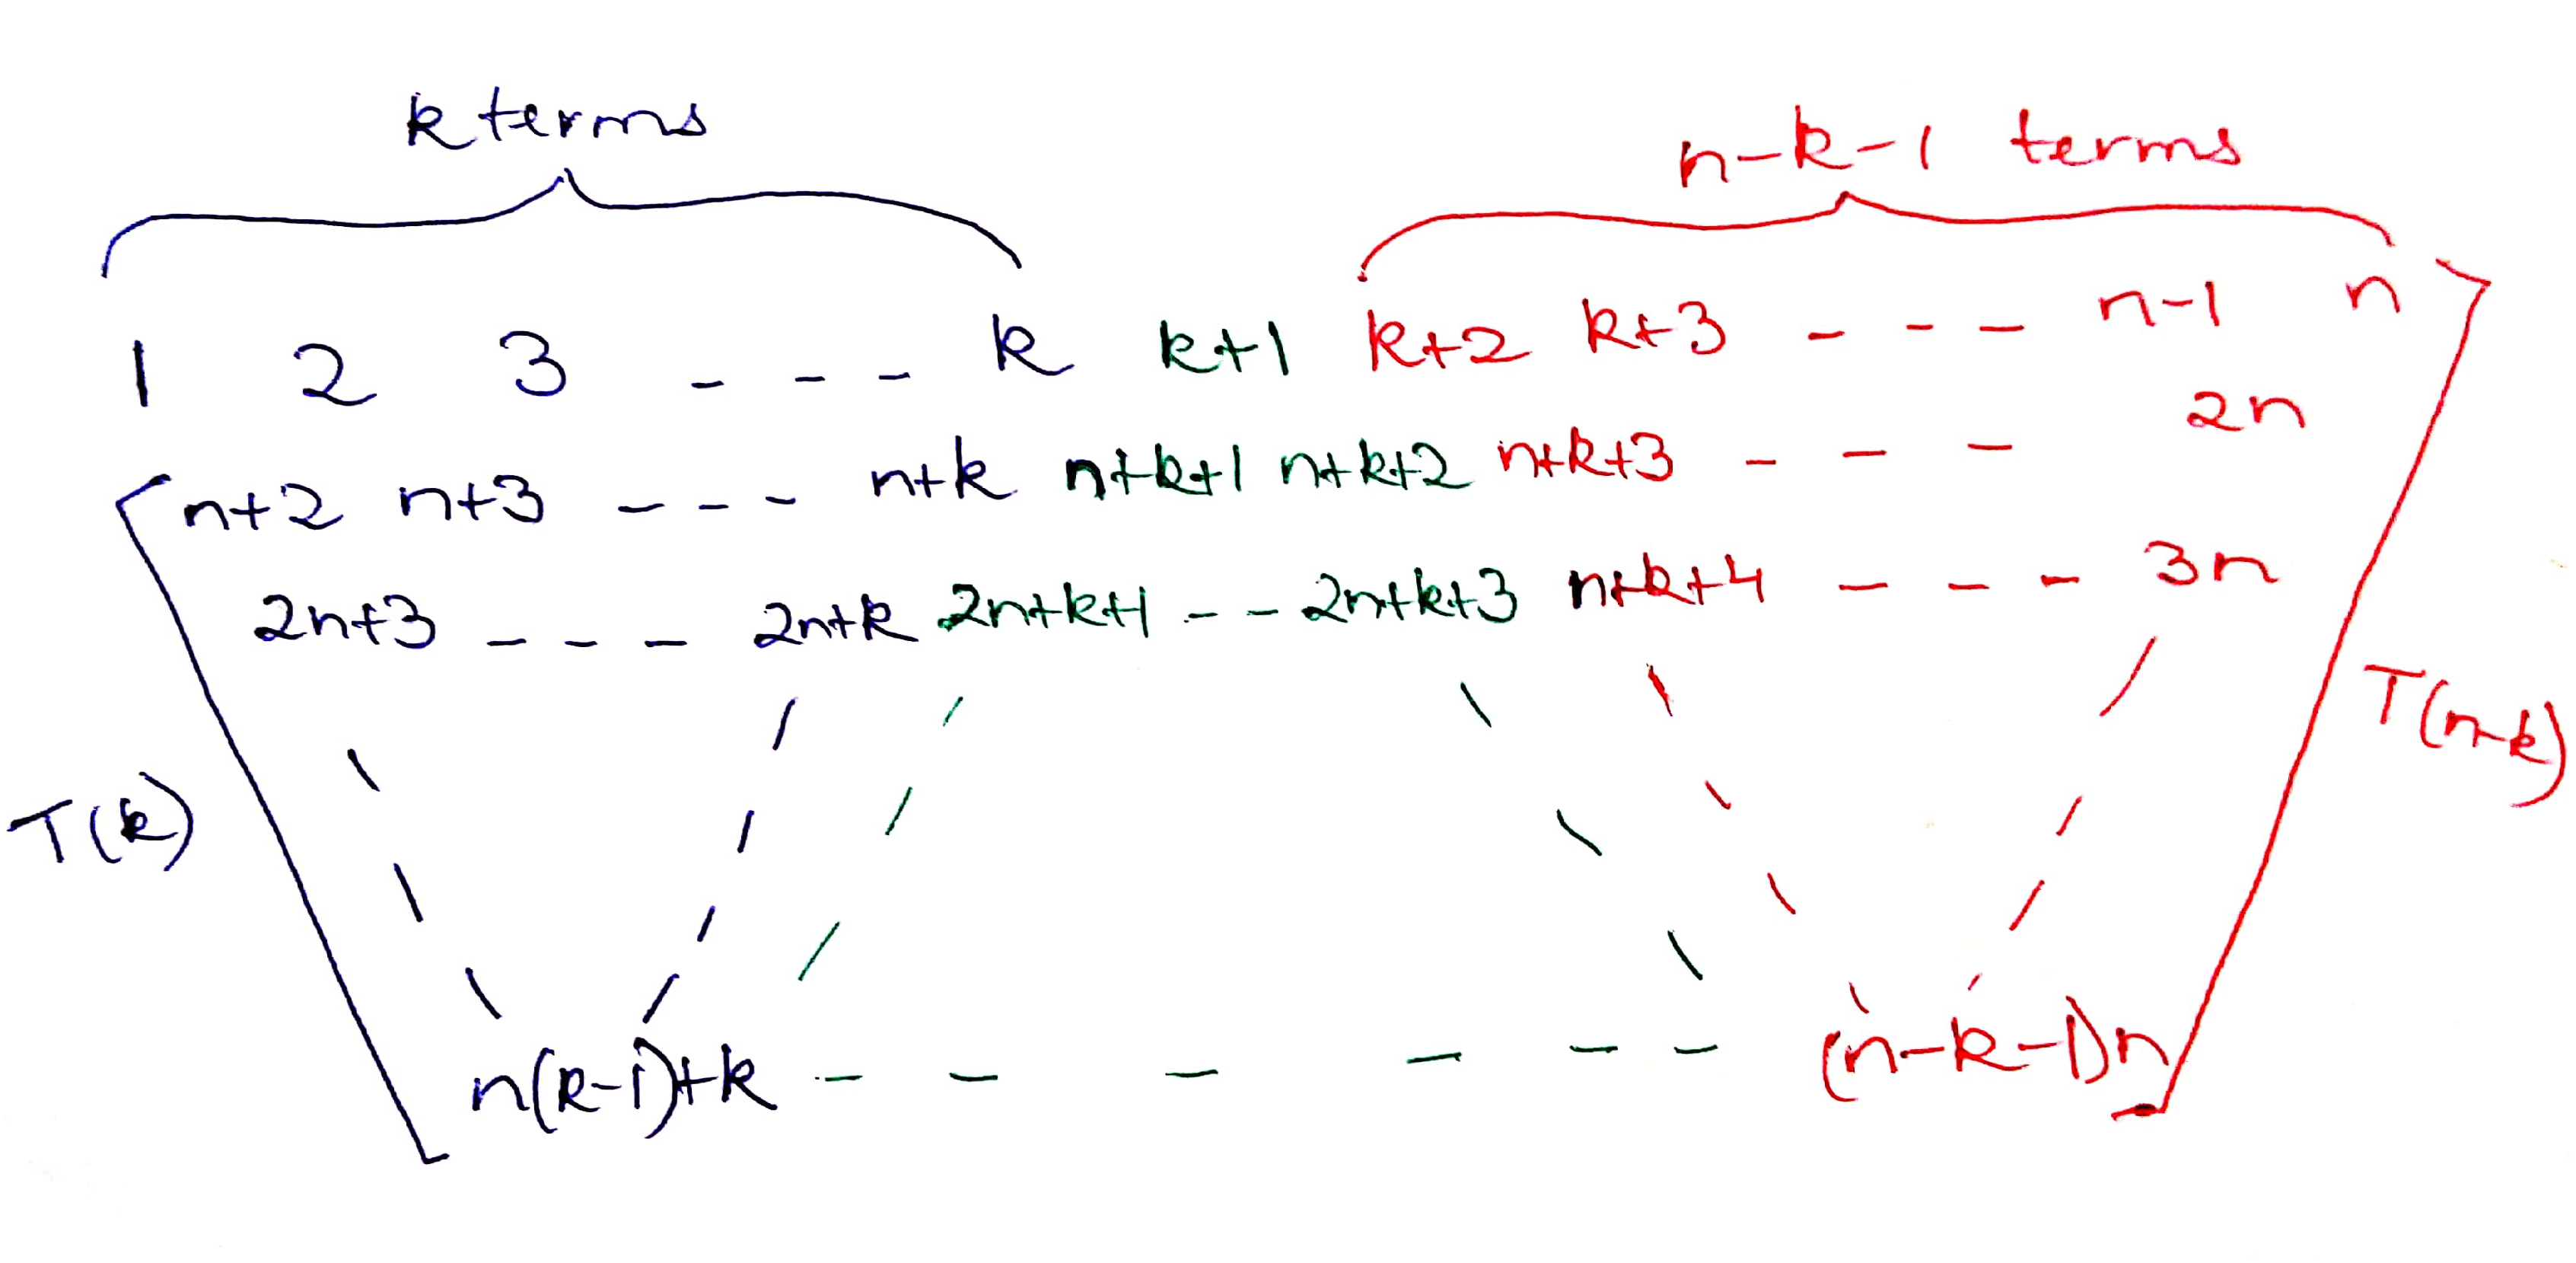
\includegraphics[scale=0.125, angle=-1]{picking.png}
  \label{fig:fig3}
  \end{figure}
  
  So, we can use the sub-tree $T'$ in red \ref{fig:fig1} to construct set T under the following conditions - 
  \begin{enumerate}
      \item Any $i \in T'$ can be in T if and only if both its parents are also in T.
      \item If $i$ has no parent nodes, it can be added to T.
  \end{enumerate}
  
  
  
  We can see that $T'$ has $k-i$ elements in it's $i$th row for $1\le i\le k-1$. We shall call such a tree $T(k)$. Thus we have, that under the above conditions, we can pick subsets $T$ from $T(k)$ in $C_k$ ways.
  
  So, for $C_n+1$, we get a tree with $n$ elements in its first row, i.e $T(n+1)$ [Figure $\ref{fig:fig3}$]. Pick the first $k$ elements from the first row and add them to set $T$. We can pick the remaining  elements from $T(n+1)$ in the following two ways -
  \begin{enumerate}
      \item Elements which are children of the $k$-elements already picked. These elements are in the form of $T(k)$, so they can be picked in $C_k$ ways.
      \item Elements excluding the first $k+1$ elements of the first row. These form a tree of the form $T(n-k)$, and can thus be counted in $C_{n-k}$ ways. 
  \end{enumerate}
  Thus, for every value of k between 0 and n, we can pick subsets T in $C_n C_{n-k}$ ways. Summing over all values of k we get,
  \[C_{n+1} = \sum_{i=0}^n C_i C_{n-i}, \qquad (n \geq 0; C_0 = 1).\]
\end{proof}

\subsection{Catalan Generating Function}

\begin{proof}
  Let \[ C(x) = \sum_{n=0}^\infty C_n x^n \]
  \begin{flalign*}
  So, C(x)^2 &= C(x)C(x) &\\
  &= (C_0 + C_1 x + C_2 x^2 + ...)((C_0 + C_1 x + C_2 x^2 + ...) &\\
  &= C_0 C_0 + (C_0 C_1 + C_1 C_0)x + (C_0 C_2 + C_! C_1 + C_2 C_0)x^2 + ... &\\
  &= C_1 + C_2 x + C_3 x^2 + ... &\\
  &= \sum_{n=0}^\infty C_{n+1} x^n &\\
  &= \frac{C(x) - C_0}{x} &&[\because x\sum_{n=0}^\infty C_{n+1} x^n + C_0 = C(x)] &\\
  \end{flalign*}
  Rearranging the equation, we get 
  \[ xC(x)^2 - C(x) + 1 = 0 \]
  Which is a quadratic equation in $C(x)$. Using the quadratic formula we get
  \[ C(x) = \frac{1 \pm \sqrt{1-4x}}{2x}\]
  Since \( C(0) = C_0 = 1 \)
  \[1 = \lim_{x\to0} \frac{1 \pm \sqrt{1-4x}}{2x} \]
  But $\lim_{x\to0} \frac{1 + \sqrt{1-4x}}{2x}$ goes to $\infty$, so
  \[ C(x) = \frac{1 - \sqrt{1-4x}}{2x}\]
\end{proof}

%...Define the Catalan number generating function and prove it satisfies the usual formula

\section{Narayana Numbers}

\begin{defn}
  The \textit{Narayana numbers} $N_{n, k}$ is the number of expressions containing n pairs of parentheses, which are correctly matched and which contain k distinct nestings. \cite{wiki:narayana}
\end{defn}

\begin{thm}
  Let $N_{n,k}$ be as in Definition 2.1. Then
  \[ N_{n,k} = \frac{1}{n}\binom{n}{k}\binom{n}{k-1}, \qquad (1 \leq k \leq n). \]
\end{thm}

\begin{proof}
  Evaluating the RHS we get
\begin{flalign*}
  N_{n,k} &= \frac{1}{n} \frac{n!}{k!(n-k)!} \frac{n!}{(k-1)!(n-k+1)!} &\\
  &= \frac{(n-1)!}{k!(n-k)!} \frac{n!}{(k-1)!(n-k+1)!} &\\
  &= \binom{n-1}{k-1} \frac{n!}{k!(n-k+1)!} &\\
  &= \frac{1}{(n+1)} \binom{n-1}{k-1} \binom{n+1}{k} &\\
\end{flalign*}
  So we see that
  \[ \frac{1}{n}\binom{n}{k}\binom{n}{k-1} = \frac{1}{n+1}\binom{n-1}{k-1}\binom{n+1}{k}\]
  Or
  \[ \frac{n+1}{n}\binom{n}{k}\binom{n}{k-1} = \binom{n-1}{k-1}\binom{n+1}{k} 
  \label{1}\tag{1}\]
  Now, 
  \[\frac{1}{n}\binom{n}{k}\binom{n}{k-1} = \frac{n+1}{n}\binom{n}{k}\binom{n}{k-1} - \binom{n}{k}\binom{n}{k-1}\]
  Hence,
  \[N_{n,k} = \binom{n-1}{k-1}\binom{n+1}{k} - \binom{n}{k}\binom{n}{k-1} \tag{From \eqref{1}}\]
  Since the RHS must be a positive integer, $N_{n,k}$ must be a positive integer.

  
\end{proof}



\bibliography{refs}{}
\bibliographystyle{alpha}

\end{document}